\section{Review of PubChem Assay 1851}
  

PubChem BioAssay 1851 contains data for inhibition of five major CYP isoforms (CYP1A2, CYP2C9, CYP2C19, CYP2D6 and CYP3A4) by 17,143 chemical compounds. \cite{Veith2009} The the tested compounds were all drugs or drug-like compounds. The chemical space revealed that the majority of compounds had molecular weight below 500 daltons and logP below 5. \cite{Lapins2013}

The assay used low low-fluorescence substrates, which are converted to more-fluorescent metabolites. The progression of the reaction is measured by an increase in fluorescence intensity during CYP metabolism of the substrate. Inhibitors of a particular CYP reduce the rate of metabolism of the substrate and this results in a decreased fluorescence signal. \cite{Zlokarnik2005}

The most recent technology developed for CYP inhibition is based on substrates that release luciferin as the metabolite. This is a coupled assay system in which addition of luciferase and ATP converts the freed luciferin to des-carboxyluciferin with light emission. The format is similar to fluoresence methods, requiring addition-only manipulations and employing luminescence plate readers. \cite{Zlokarnik2005}

The assay obtained lumiescence readings at a range of compound concentrations.Fi Here I need a paragraph describing the Hill equation and its suitability for curve fitting

%Inorganic compounds, non-covalent inhibitors and compound mixtures were removed from the dataset, leaving 16,359 compounds. \cite{Lapins2013}

In the dataset, compounds are classified as active or inactive inhibitors for each CYP with an activity cutoff set to AC50 = 10uM (AC50, “activity concentration 50”, refers to the concentration that is required to elicit half-maximal effect). However, in cases where the dose-response curve for a compound showed poor fit or the inhibition efficacy was below 60\%, the assay results were regarded as inconclusive.\cite{Lapins2013}

Compounds were characterized by their Activity Score and regarded as inhibitors if their activity score ranged between 40 and 100. PubChem Acitivity Score is assigned based on an AC50 values, which was combined with a confidence measure. Combining measures for completeness of a dose-response curve and efficacy of inhibition, resulted in the Activity Score, where a larger value indicates higher inhibitory activity and/or higher confidence in inhibitory assay result. Compounds with an activity score equal to zero are considered as non-inhibitors while compounds with activity scores above 0 and up to 40 are considered inconclusive. \cite{Lapins2013}

The data from Pubchem Assay 1851 is available for download from the NIH website. The interface changes from time to time, but I downloaded two files which comprised the entire dataset for the experiment. The first file, a structures file, contained the structural information encoded in the simplified molecular-input line-entry system (SMILES) format for each tested compound with corresponding Structure ID (SID) and Compound ID (CID) as assigned by NCBI. Another file, also organized by SID and CID, contained all of the luminescent responses from the high-throughput screen and the fitted parameters that are summarized by the activity score. 

\begin{figure}[!htp]
  \caption{dataset preparation}
  \centering
\includegraphic

\subsection{results}
The results of this large-scale screening against five CYP isoforms identified that the majority of compounds in a typical chemical library cross-inhibited several isoforms, while only a small fraction of the compounds did not inhibit any of the isoforms. \cite{Veith2009}x


\begin{figure}[!htp]
  \caption{Supervised Learning Scheme for Clasification}
  \centering
   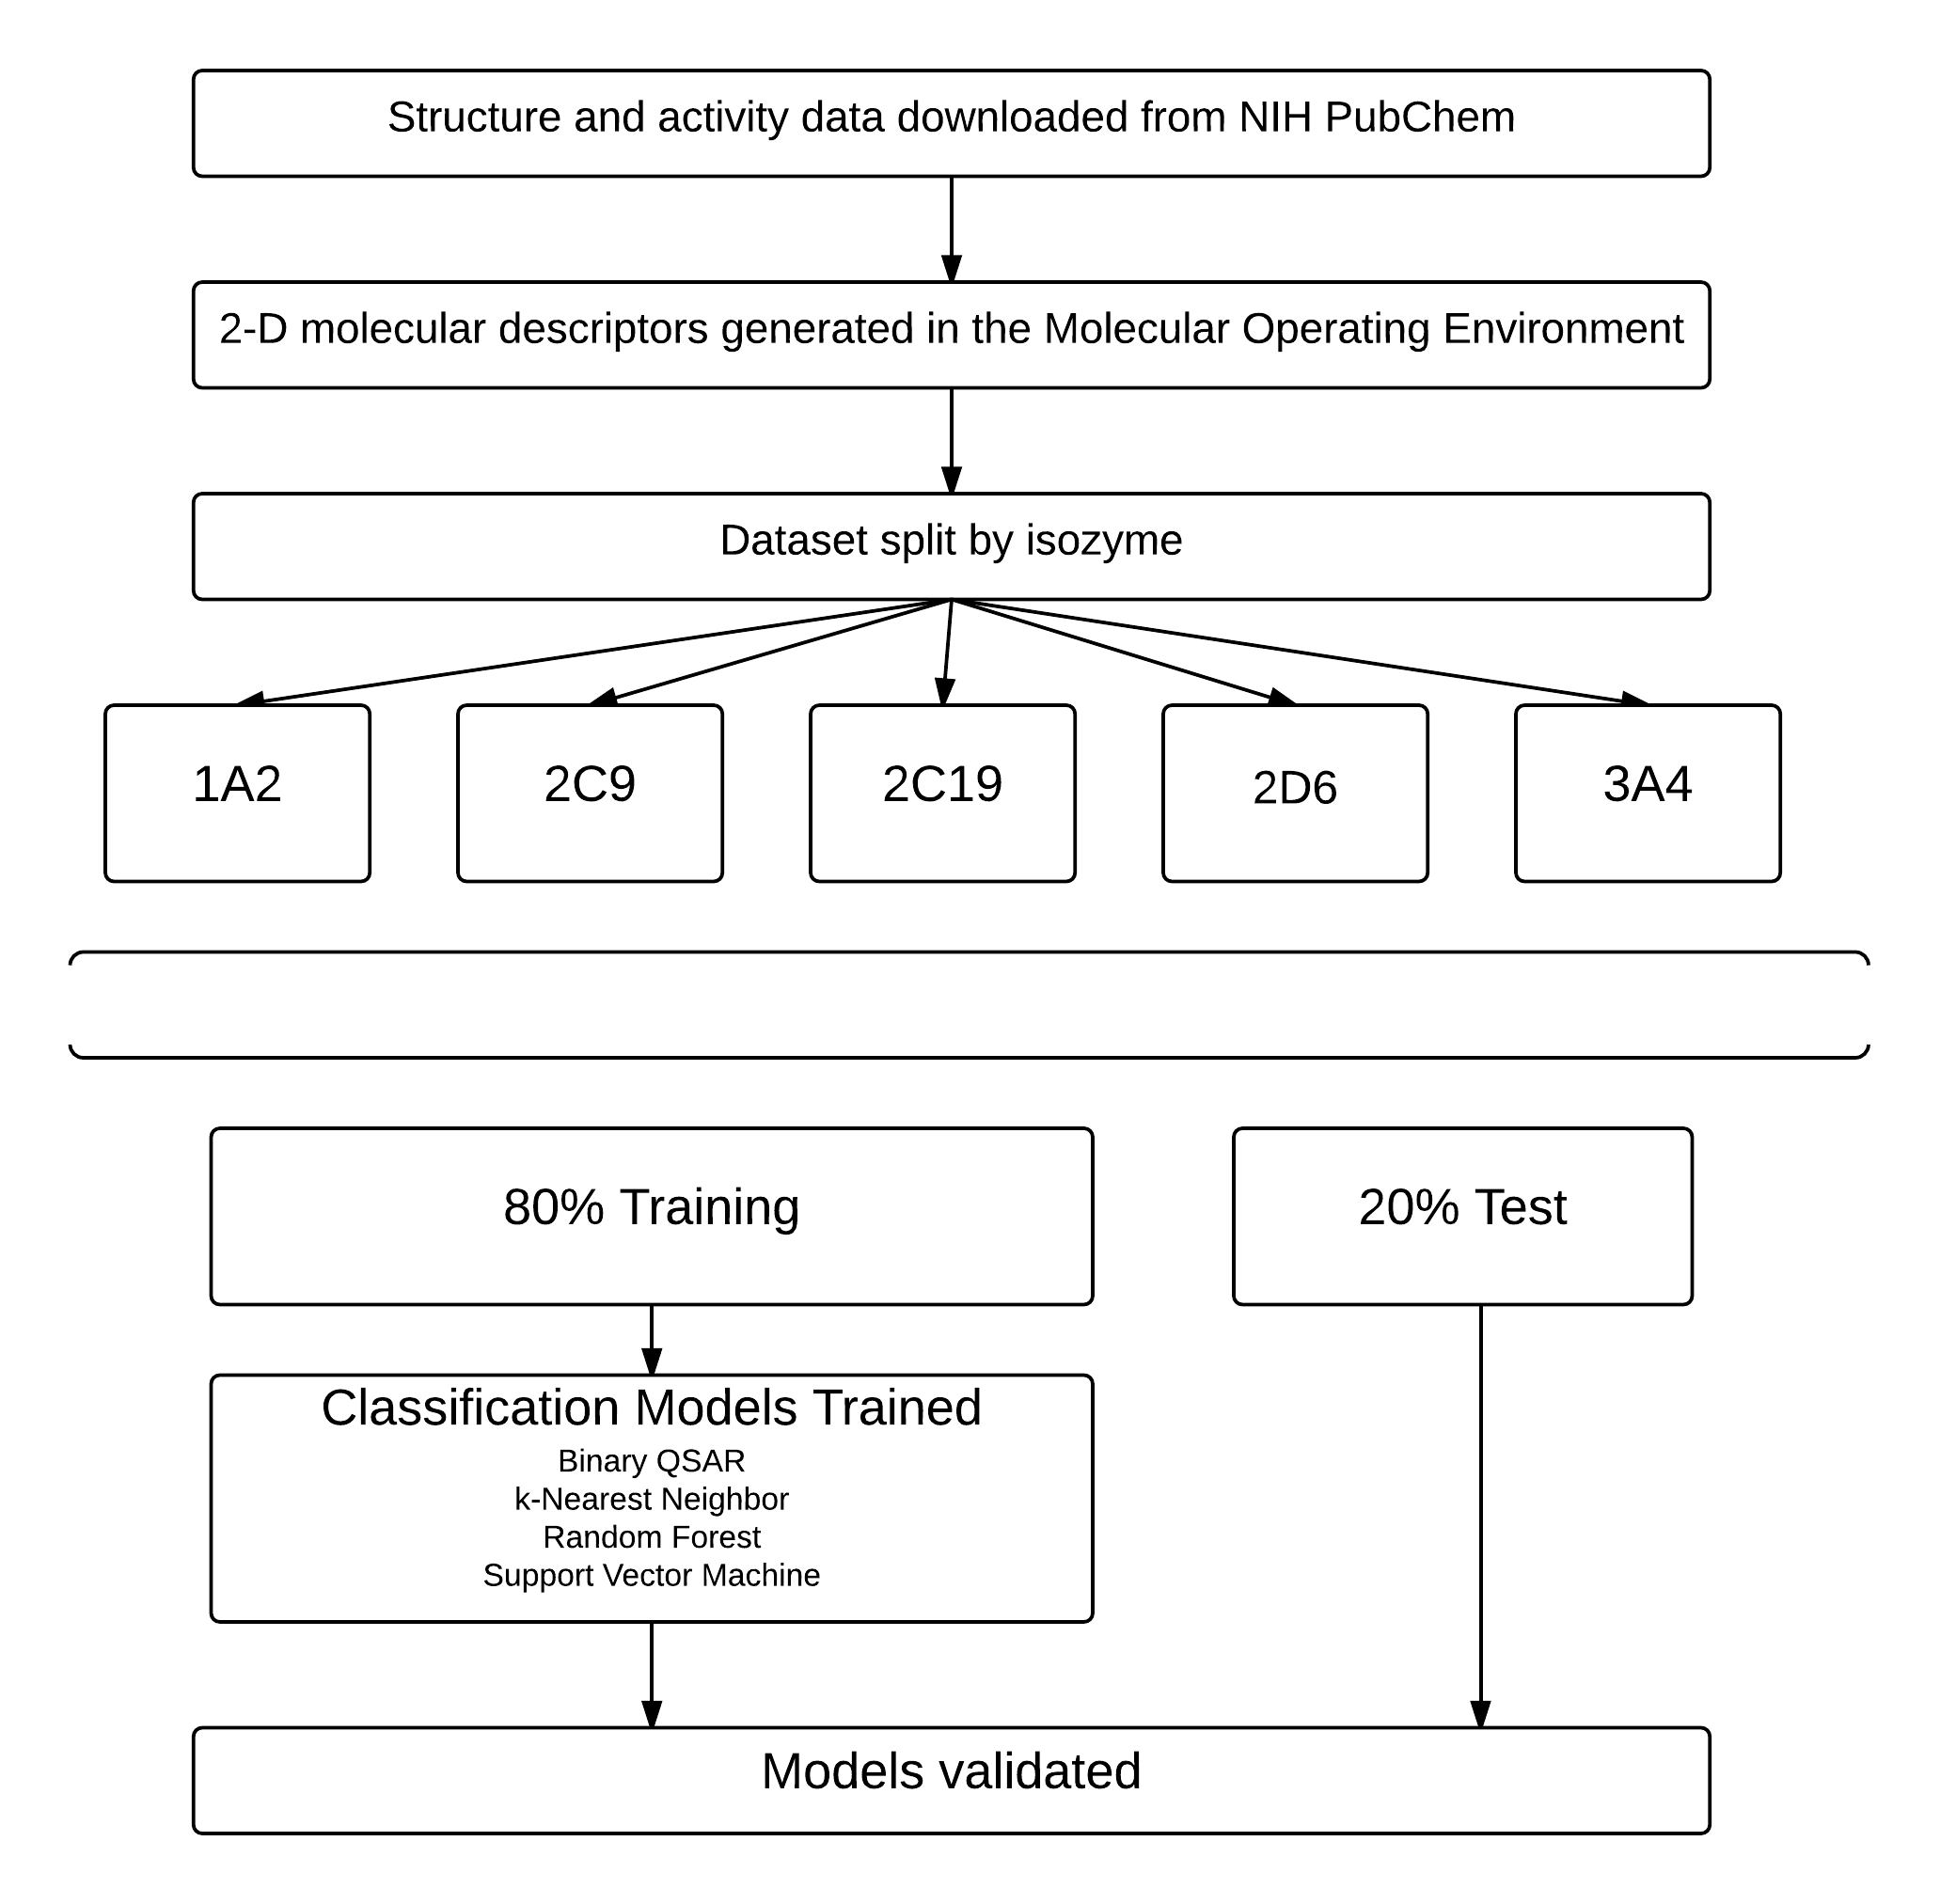
\includegraphics[width=1\textwidth]{../img/Supervised_Workflow.png}
\end{figure}


\section{Feature generation and molecular descriptors}

Data preprocessing - The preliminary steps in data preprocessing typically requires data cleaning as raw data often contain anomalies, errors, or inconsistencies such as missing data, incomplete data, and invalid character values which may cause trouble in data analysis if left untreated. It is more complicated when data are collated from many formats requiring harmonization and elimination of redundancies.\cite{Nantasenamat2009}

There exists a great deal of variability in the range and distribution of each variable in the data set. However, this may pose a problem for algorithms using distance measurements in the learning step. These situations are handled by applying statistical techniques such as min-max normalization or z-score standardiation. 

In min-max normalization, the minimum and maximum value of each variable is adjusted to a uniform range between 0 and 1 according to the following equation: xxxxxx In z-score standardization, essentially the variable of interest is subjected to statistical operation to achieve mean center and unit variance according to the following formula: xxxxxx \cite{Nantasenamat2009}

In situations where the data does not have a Gaussian (normal) distribution, simple mathematical functions can be applied to achieve normality or symmetry in the data distribution. A commonly used approach is to apply logarithmic transformation on the the variable of interest in order to achieve distribution approaching normality. This is typically performed on dependent variables such as the modeled biological/chemical properties of interest whereby IC50 may be transformed to logIC50 or -logIC50. Practically, such mathematical operation is applied to each individual value of a given variable of interest. \cite{Nantasenamat2009}

Feature or variable selection -- Typically data sets often contain redundant or noisy variables which make it more difficult for learning algorithms to discern meaningful patterns from the input data set. ... Such multicollinearity of the variables ... treated ... in order to reduce unnecessary computational resources that are required in model construction. \cite{Nantasenamat2009}

Statistical evaluation In QSAR modeling it is essential to validate the model as well as apply statistical parameters to evaluate its predictive performance. The predictive performance of a data set can be assessed by dividing it into a training set and a testing set. The training set is used for constructing a predictive model whose predictive performance is evaluated on the testing set. Internal performance is typically assessed from the predictive performance of the training set while external performance can be assessed from the predictive performance of the independent test set that is unknown to the training model. A commonly used approachfor internal validation is known as N-fold cross-validation where a data set is partitioned into N number of folds. For example, in a 10-fold cross-validation 1 fold is left out as a testing set while the remaining 9 folds are used as the training set for model construction and then validated with that fold left out. In situations where the number of samples is limited, leave-one-out cross-validation is the preferred approach. Analogously, the number of folds is equal to the number of samples present in the data set. \cite{Nantasenamat2009}

Some standard measures of performance used for QSAR models are sensitivity, specificity, positive predictivity, negative predictivity, and concordance. Additional measures such as the Matthews coefficient can be used as a single metric for comparing one model to another while correcting for bias. Because most stat models can be modified to have greater specificity vs sensitivity (or vice versa) by adjusting the training set or applying predictive filters, the Matthews coefficient can be used to determine when the modification is so extreme that it leads to overall degradation of the models’ performance.\cite{Kruhlak2012}

%Statistical parameters - Pearson's correlation coefficient (r) is a commonly used parameter to describe the degree of association between two variables of interest. Calculated r values have values between -1 and +1 which indicate direct (positive) and indirect (negative) correlation. For describing the relative predictive performance of a QSAR model, r is used to measure the correlation between experimental (x) and predicted (y) values of interest in order to observe the variability that exists between variables. This is calculated according to the following equation: ...

%Root mean squared error (RMS) is another commonly used parameter for assessing the relative error of the QSAR model. RMS is computed according to the following formula: ...

%F-test -- The statistical significance of QSAR models are typically assessed by performing an ANOVA and observing the calculated F values, which is essentially the ratio between the explained and unexplained variance. Comparison between multiple QSAR models can be performed when all models have the same number of degrees of freedom meaning that the same sets of compounds and descriptors are used. Each model yields a calculated F value and the best performing model is identified as those bearing the highest value.\cite{Nantasenamat2009}

Degrees of freedom take into consideration the number of compounds and the number of independent variables that are present in the data set. This can be calculated using the equation n - k - 1 where n = \# of compounds k = \# of descriptors. The higher the value, the more reliable the QSAR model is. \cite{Nantasenamat2009}

Mathematically speaking, an outlier is essentially a data point which has a high standard residual in absolute value when compared to other samples in the data set. A commonly used approach for detecting outliers is performed by calculating the standard residuals of all compounds in the data set of a QSAR model. \cite{Nantasenamat2009}



\section{Data analysis consideration}
\begin{description}
\item Balance number of positives and negatives

\item Split dataset into training and test set before looking at it.

\item Cross-validation
\end{description}

\begin{description}
\item Molecular Operating Environment
\item SciPy ecosystem

\end{description}


\subsubsection{Modeling in Python}
The Python programming language is a dynamically-typed, object-oriented interpreted language. Its primary strength lies in the ease with which it allows a programmer to rapidly prototype a project, although it also has a powerful and mature set of standard libraries that can facilitate large-scale production-level software engineering projects as well. Python has a very shallow learning curve and excellent online learning resources.


\subsubsection{Methods of Correlation of Compound and CYP Descriptors to Activity Data}

\subsubsection{$\kappa$-Nearest Neighbor ($\kappa$NN}
The kNN algorithm predicts the class of a test set object based on the class membership of its $\kappa$ most similar training set objects. \cite{Lapins2013}

\subsubsection{Random Forest (RF)}
Random Forest is a classifier that consists of multiple decision trees. A decision tree is made of nodes and branches. At each node the dataset is split based on the value of some attribute that is selected so that the instances of different classes are predominately moved to different branches. 

Classification starts at the root node and is performed by passing the instances along the tree to leaf nodes. \cite{Lapins2013}

To introduce diversity between the trees of a random forest, a small subset of all attributes is randomly selected to take decisions at each node of each tree. The classification decision is performed by considering results of all trees by majority vote. The optimal size of the forest and the number of attributes to consider at each node were found by performing five-fold cross-validation. \cite{Lapins2013}

\subsubsection{Support Vector Machines (SVM)}
SVM is a machine learning technique for classification or regression that uses linear or non-linear kernel-functions to project the data into a high-dimensional feature space. \cite{Lapins2013}

Correlation is performed in this hyperspace based on the structural risk minimization principle i.e., aiming to increase the generalization ability of a model. \cite{Lapins2013}

They applied the commonly used Gaussian radial basis function kernel optimal gamma (width of the kernel function) and error penalty parameter C were found after performing grid search on five­fold cross validation. \cite{Lapins2013}

\subsubsection{Binary QSAR in MOE}


